\chapter{Ausarbeitung des Architekturkonzepts}\label{chap:concept}
\section{Analyse der bisherigen UI-Struktur}
Momentan werden alle für die Darstellung der verschiedenen Ansichten benötigten Parameter und Metadaten in einzelnen Dateien als Teil des Solution-Verzeichnis gespeichert. <Ansichtsname>.dli enthält die Konfiguration für die Detailansicht und <Ansichtsname>.vlc die Konfiguration der Übersichtsliste. Für den Aufbau dieser Dateien existiert leider keine offizielle Spezifikation und auch keine Dokumentation, es ist daher eine Herausforderung direkt alle nötigen Informationen aus ihnen auszulesen und bedarf unter Umständen spätere Anpassungen am Auslesetool oder der künftigen Struktur.

\subsection{DLI}
\subsection{VLC}
\subsection{Neue Struktur}
Der Aufbau der neuen Struktur entspricht simplen JSON-Daten. 
% wird auf dem server gespeichert und dient dann direkt auch als langzeitspeicher für die UI (kann in DB serialisiert werden, Änderungen nur auf Clientseite)
% enthält position im grid, anfangs durchnummeriert, später mit von user gesetzten werten

\section{Client}
% react skelett mit komponenten wird ausgeliefert -> aufbau ui dann dynamisch

\subsection{React-Komponenten}
Die jetzige Oberfläche besteht aus einer festen Anzahl von Darstellungs-Elementen welche je nach Kontext andere Inhalte anzeigen. Zu den Elementen gehören unter anderem statische Texte, Eingabefelder, Check- und Comboboxen, Gruppierungen und Container für weitere Elemente. Der Kontext für den Inhalt ergibt sich aus dem Datenbankfeld das mit dem jeweiligen Element verknüpft ist und Einstellungen wie Sichtbarkeitsbedingungen oder Formatierungen. Da bereits im Voraus bekannt ist, welche Art von UI-Elementen benötigt werden, können diese auch schon im Vorfeld erstellt werden. Diese fertigen React-Komponenten werden mit dem Produkt ausgeliefert und können zur Laufzeit dynamisch auf der Webseite platziert werden. Die Funktionalität dieser Elemente orientiert sich dabei immer an der Funktionalität der Originalkomponente.
% props auflisten (evtl. nur gemeinsame?)

\subsection{Verwendung der Komponenten}
% => nicht nur Elemente sondern auch Anordnung wichtig!!
\subsubsection{Erste Layout-Überlegungen}
Zu Beginn erschien die zentrale Frage, wie  es technisch möglich ist, die Komponenten der Detailansicht vom Benutzer anpassbar anzuordnen. Eine naive Herangehensweise kann in Abbildung~\ref{fig:layout_grid_test} gesehen werden. Umgesetzt wurde dies mit einem CSS-Grid (rote Umrandung) das entweder horizontal oder vertikal in zwei Hälften getrennt werden kann. Jede dieser Hälften stellt abermals ein CSS-Grid dar das beliebig zwischen Elterncontainern verschoben werden kann. Abstrakt handelt es sich bei diesem Ansatz um einen nicht balancierten binären Baum an dessen Endpunkten (Blätter) sich genau eine UI-Komponente (blaue Umrandung) befindet. Es wurde schnell klar dass diese Lösung in ihrer binären Form nicht flexibel genug ist um vorhandene Layouts abzubilden. Da ein Ausbau auf eine Struktur mit variabler Anzahl an Verzweigungen sehr komplex und zeitaufwändig gewesen wäre wurde der Ansatz gänzlich verworfen und nach einer Alternativen Lösung gesucht. \fixme{bessere erklärung und begründung warum nicht flexibel genug}

\begin{figure}
    \centering
    \captionsetup{justification=centering}
    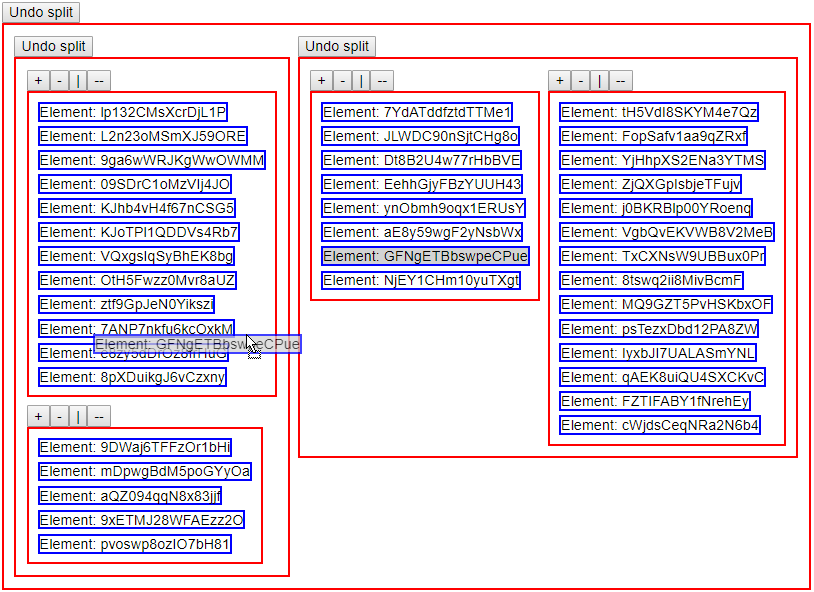
\includegraphics[width=\textwidth]{figures/layout_grid_test.png}
        \caption{Eigener Layout-Prototyp mit CSS-Grids}\label{fig:layout_grid_test}
\end{figure}

% Grid / Table

\subsection{Identifikation auf Server}
Um die UI-Elemente mit Daten aus der Datenbank zu befüllen muss eine entsprechende Identifikation möglich sein. Es wird vorausgesetzt dass diese eindeutige ID, ob sie aus Tabellennamen plus Spaltenname der Datenbank oder aus anderen Informationen besteht, zum Zeitpunkt der Übersetzung einer Ansicht bereits bekannt ist und mit ausgelesen werden kann. Bei Anfragen an den Server werden alle IDs der beteiligten Elemente mit an den Server übertragen, ebenso wie dieser bei Antworten immer die IDs der Elemente, für welche die Antwortdaten gedacht sind, sendet.

\subsection{Visualisierung von Lade- und Fehlerzustände}
Direktes Feedback ist für die subjektive Einschätzung einer performanten Webseite essentiell. Typischerweise ist die am längsten dauernde Aktion auf einer Webseite das Nachladen von Daten, es ist also sinnvoll diesen Vorgang für Nutzer visuell ansprechend deutlich zu machen. Für diesen Zweck sollen alle React-Komponenten eine visuell simplere Repräsentation von sich selbst in Form von unspezifischen grauen Boxen enthalten, welche nur auf die ungefähre Form und Darstellung mit Echtdaten hindeutet und die bereits während des Ladevorgangs angezeigt werden kann. In Abbildung~\ref{} sieht man eine Gegenüberstellung der beiden Repräsentationen (finaler Zustand links, Ladezustand rechts), jeweils für ein Edit-Element und ein Checkbox-Element.

Mit einer entsprechende Einfärbung und einem Hinweistext kann diese Visualisierung, wie in Abbildung~\ref{} an zwei unterschiedlichen Ausführungen gezeigt (normaler Zustand links, Fehlerzustand rechts), ebenfalls dazu genutzt werden um Fehlerzustände beim Laden von Daten zu signalisieren.

\subsection{Einbindung von GraphQL mit Apollo}
% integration erklären: queries so weit wie möglich trennen und zu jeder Komponente speichern

\subsection{Editier-Modus}
% immer.js

\subsection{Individualisierung}
% layout und aussehen -> auf server serialisieren

\subsection{Suche, Filter, Sortierung}
% mit table lib erledigt

\subsection{Tests und Continuous Integration}

\section{API}

% copy of api contract from api itself => bei graphql gegeben
\subsection{GraphQL-Schema} % struktur und daten
\subsection{Keine Business Logik im Client}
